\section{System Perspective}
\label{sec:sys_perspective}

\subsection{Requirements}
\label{sec:reqs}

The functional requirements are:
\begin{enumerate}
    \item The \textit{Minitwit} system shall have the same functionality as the original \textit{Minitwit} system.
    \item The \textit{Minitwit} system shall expose an API that meets the \textit{Simulator's} specification.
\end{enumerate}

The non-functional requirements are:
\begin{enumerate}
    \item The system shall be written in Go using the Gorilla framework and JavaScript using the React library.
    \item The system shall be hosted on DigitalOcean Droplet instances.
    \item The system shall be accessible by end-users independent of operating system.
    \item Users with experience from other chat services such as Twitter should be able to post a tweet/message.
\end{enumerate}

\subsection{Design and Architecture}
\label{sec:design_arch}
% Design of your ITU-MiniTwit systems
% Architecture of your ITU-MiniTwit systems
% Important interactions of subsystems

The requirements of the \textit{Minitwit} system are well-defined. Hence, the design of the system is limited to the selection of the three-tier architecture.
\autoref{des-and-arch:fig:three-tier-arch} below depicts this architecture applied to the \textit{Minitwit} system.

\begin{figure}[H]
    \centering
    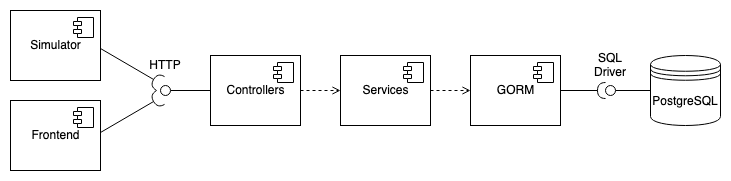
\includegraphics[width=\textwidth]{images/DevOpsArch.png}
    \caption{A high-level overview of \textit{Minitwit's} three-tier architecture}
    \label{des-and-arch:fig:three-tier-arch}
\end{figure}

Each layer is discretely bounded by communication interfaces.
The first layer consists of two clients to the \textit{Minitwit} system.
The frontend allows end-users to interact with the system, and the simulator replicates live users interacting with the system.
The second layer provides the core functionality of the \textit{Minitwit} system.
It exposes this functionality through two HTTP APIs, for the frontend and simulator respectively.
The third layer is a PostgreSQL database that provides the system with persistent data.

To implement the \textit{Services} component there is an important interaction with the \textit{GORM} component. \textit{GORM} is an object-relational mapper for Golang. The \textit{Services} component uses it as a bridge pattern to add a layer of abstraction such that several database vendors can provide persistence functionality.
\autoref{des-and-arch:fig:bridge-pattern} below reveals how the use of different SQL drivers allows \textit{Minitwit} to support different database vendors.

\begin{figure}[H]
    \centering
    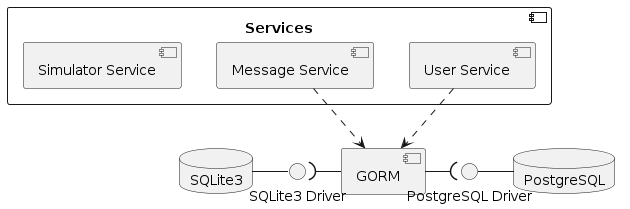
\includegraphics[scale=0.65]{images/DevOpsBridge.png}
    \caption{An illustration of \textit{Minitwit's} bridge pattern to support different database vendors}
    \label{des-and-arch:fig:bridge-pattern}
\end{figure}



\subsection{Dependencies}
\label{sec:deps}
To boost developer productivity the \textit{Minitwit} system uses Go's own dependency management system to import third-party packages.
A noteworthy package we depend on is the \textit{Gorilla} package.
It provides functionality to implement the HTTP APIs required by the functional requirements, such as a multiplexer and session management. 
\autoref{deps:fig:depth1} overleaf is a visualization of the Go package dependencies of \textit{Minitwit} with a depth of one.
We have also generated a complete list and complete visualization (see \autoref{app:go-pkg-deps}).

\begin{sidewaysfigure}
        \centering
        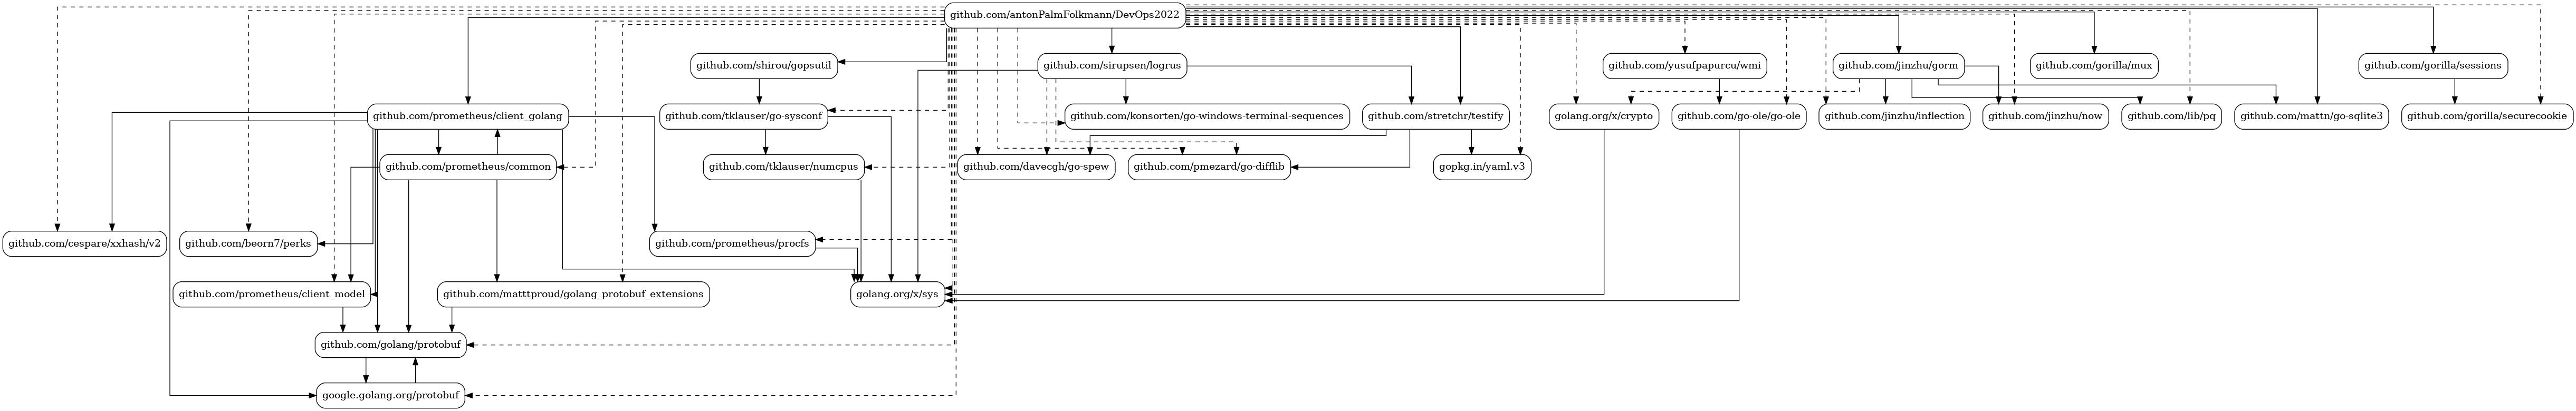
\includegraphics[width=\textwidth]{images/depth-1-deps.jpg}
        \caption{An graph of Minitwit's immediate dependencies. A full resolution can be found here \href{https://raw.githubusercontent.com/antonPalmFolkmann/DevOps2022/main/report/images/depth-1-deps.jpg}{here}.}
        \label{deps:fig:depth1}
\end{sidewaysfigure}

\newpage
To package the application we depend on Docker. To provision environments we use DigitalOcean's CLI tool \textit{doctl}.
By using Docker we can encode dependencies in the form of layers for the image.
Notably, the base layer of the \textit{Minitwit} system is the Golang 1.17 image.
We take advantage of \textit{doctl}'s ability to programmatically provide environments with Docker preinstalled.
In this way we can be sure that any environment we provision can run the \textit{Minitwit} application, since it is packaged with Docker. 
A complete list of our production environments dependencies can be found in \autoref{app:prod-deps}.


\subsection{Current State of the System}
\label{sec:current_state}
The system has evolved to be more scalable, maintainable, and reliable.
The system can scale with multiple users sending simultaneous requests by taking advantage of Gorilla's multi-threaded multiplexer.
Scalability and reliability is delivered by replicating the \textit{Minitwit} system across multiple physical nodes using Docker swarm.
Additionally, we have introduced continuous integration (CI) pipelines to ensure the reliability of the system.
Finally, the system has been made more maintainable.
The system is observable through features such as logging and monitoring, and updating the system has been eased through our continuous delivery (CD) pipeline.

The maintenance work is still not complete, and some top priority improvements are:
\begin{enumerate}
    \item Implement the ability to flag tweets.
    \item Update Go dependency to the latest version (to Golang 1.18).
    \item Add more indexed fields log messages to add more granularity when filtering and searching for log messages.
\end{enumerate}

\subsection{Licensing}
During the development of the application the project was licensed under the Massachusetts Institute of Technology (MIT) open-source license. The motivation for using the MIT license was its lack of restrictions regarding distribution, along with its compatibility with many other licenses. Most of the application’s direct dependencies’ licenses are permissive licenses such as BSD, Apache, ISC and other MIT licenses. However, during the report writing phase of the project, it has come to the team’s attention that some dependencies are licensed under the Mozilla Public License (MPL). Due to the MPL being classified as a weakly protective license, licensing the project under the MIT license is not restrictive enough. As a result, the project should be re-licensed under the MPL to comply.
